\documentclass[conference]{IEEEtran}
\IEEEoverridecommandlockouts

\usepackage[utf8]{inputenc}

\usepackage{cite}
\usepackage{amsmath,amssymb,amsfonts}
\usepackage{algorithmic}
\usepackage{graphicx}
\usepackage{textcomp}
\usepackage{xcolor}
\usepackage{siunitx}
\usepackage{hyperref}
\usepackage[noabbrev, capitalize]{cleveref}
\usepackage{bm}
\usepackage{tabu}
\usepackage{booktabs}
\usepackage{subfig}
\usepackage{bookmark}
\usepackage{dsfont}

\begin{document}

\title{
    Extrinsic Calibration of 2D Laser Range Finders \\
    using Planar Features
}

\author{\IEEEauthorblockN{Bernardo Lourenço}
\IEEEauthorblockA{\textit{Departamento de Engenharia Mecânica} \\
\textit{Universidade de Aveiro}\\
Aveiro, Portugal \\
bernardo.lourenco@ua.pt}
\and
\IEEEauthorblockN{Paulo Dias}
\IEEEauthorblockA{\textit{IEETA} \\
\textit{Universidade de Aveiro}\\
Aveiro, Portugal \\
paulo.dias@ua.pt}
\and
\IEEEauthorblockN{Miguel Riem Oliveira}
\IEEEauthorblockA{\textit{Departamento de Engenharia Mecânica} \\
\textit{Universidade de Aveiro}\\
Aveiro, Portugal \\
mriem@ua.pt}
}

\maketitle

\begin{abstract}
    2D Laser Range Finders, or 2D-LRFs, are essential sensors in the field of robotics, providing accurate range measurements with high angular resolution. These sensors can be assembled on top of systems which, by granting additional degrees of freedom to the movement of the LRF, enable the 3D reconstruction of a scene. The reconstruction procedure consists of the concatenation of each scan in a single point cloud representation. To do so, the extrinsic transformation between the LRF and the motorized system, in this case, a Pan-tilt unit, must be known with high accuracy, otherwise, the quality of the 3D reconstructed point clouds is insufficient.
    In this work, a calibration procedure which determines this transformation is proposed. The method does not require a dedicated marker, which is commonly necessary and has numerous disadvantages. Qualitative inspections show that the proposed method is able to significantly reduce artifacts which typically appear on uncalibrated point clouds. Furthermore, quantitative results demonstrate that the calibrated point cloud represents the geometries present in the scene with much higher accuracy when compared with the uncalibrated point cloud.
\end{abstract}

\begin{IEEEkeywords}
LRF, calibration, reconstruction, point cloud, optimization
\end{IEEEkeywords}

\section{Introduction}\label{section:introduction}

Laser Range Finder, or LRFs, is one of the most important sensors in the field of robotics, employed in applications such as Simultaneous Localization and Mapping~\cite{cadena16} and 3D reconstruction~\cite{saito10}. Their use is increasing due to several factors, such as decreasing costs, new research and development, and a fundamental role in emerging technologies such as autonomous driving.

In this paper, a 2D-LRF is used in a 3D reconstruction system, to produce high-detail and accurate models of real scenes. Using a 2D-LRF is this system has the advantage of being several times cheaper than commercial 3D laser scanners~\cite{dias06}. The common solution involves the integration of the LRF on a turntable~\cite{maurelli09} or a Pan-tilt unit, or PTU~\cite{klimentjew09}, to enable a full 3D reconstruction. One of the challenges of this approach is the calibration of the position of the LRF, relative to the coordinate frame of a dynamic kinematic chain, such as a PTU. This process is known as the LRF-PTU extrinsic calibration.

This calibration is utterly necessary because any error introduces a shift on the position of each point, which in turn can be seen as deformations on the point cloud resulting from the acquisition. Such deformation can be seen in \cref{fig:deformed-pointcloud}, which is shown as multiple misalign planes. These deformations have a significant impact on subsequent point cloud processing methods, that rely on the accurate representation of the 3D environments, i.e. registration (for example, ICP), segmentation and feature extraction algorithms. 

\begin{figure}[h]
    \centering
    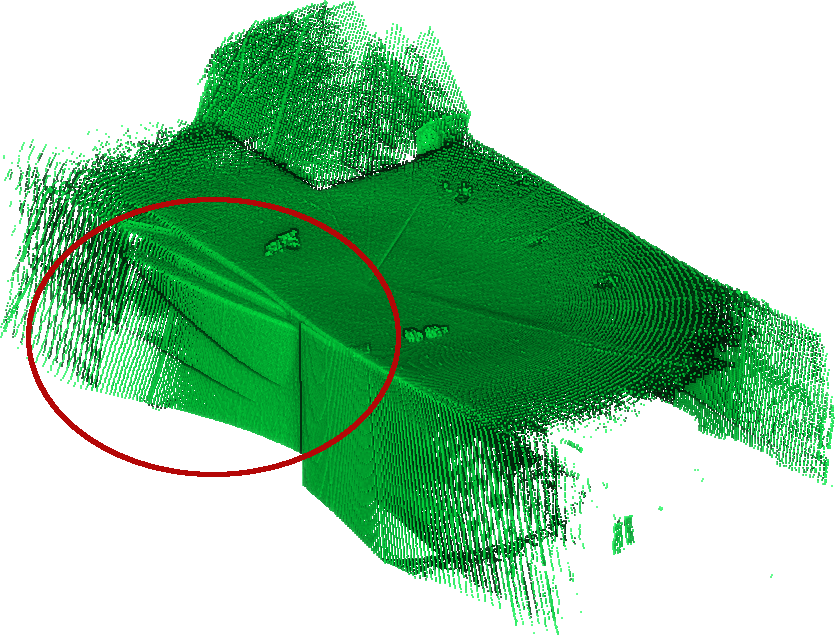
\includegraphics[width=8cm]{images/bad-pointcloud.png}
    \caption{Example of deformed point cloud, product of an inaccurate calibration of the LRF. The points where this deformation is most visible is marked in red.}
    \label{fig:deformed-pointcloud}
\end{figure}

Typically, a possible solution to do this calibration relies on a study of the geometry of such a system, using a measuring instrument, for example, a tactile Coordinate Measuring Machine. However, this approach has several disadvantages: it is time-consuming, the instruments required are expensive and generally not easily available.

Therefore, reliable and automatic methods for the LRF extrinsic calibration are required. In this field, there are two main approaches, depending on the sensor which the LRF is calibrated relative to. The first method and the most studied is the calibration of the LRF relative to a camera~\cite{chen16,vasconcelos12}, or cameras~\cite{haeselich12}. In this method, the static transformation between these two sensors is determined and relies on a correspondence between visual features captured by the camera and geometric features captured by the LRF. This features might be markers placed on the field of view of both sensors, such as a chessboard, in the case of \cite{kassir10}. However, these methods have some disadvantages in the case of LRF mounted on robotic arms: first, they require the inclusion of a camera in the system; secondly, the calibration of the camera has to be performed; and lastly, the error of both calibrations is combined during the reconstruction, which increases the inaccuracies of the final reconstruction. 

Another approach is to calibrate the 2D-LRF directly against a moving platform~\cite{zeng18}. Most of these methods rely on the comparison between the structure of the reconstructed points with an object with a known 3D geometry, such as a plane, a ball~\cite{pereira16} or a cone~\cite{almeida12}. In~\cite{kim13}, a marker formed by two perpendicular planes is used, and their points are segmented from the reconstructed point cloud. Then, the relation between the normals of these planes is used as the objective function for the calibration. However, this method presents some limitations: first, ensuring that two planes are perpendicular with a small error can be very hard (it requires a well-built marker); second, it is not straight-forward how to increase the number of planes; finally, by using a small marker, only a small portion of the space is occupied, which means that only a portion of the sensors' full field of view is used, which may lead to a sub-optimal result.

\section{Problem Formulation}\label{section:problem-formulation}

The 2D-LRF is a sensor that outputs several laser scans. Each laser scan is a set of range measurements taken sequentially along several directions all coincident with a plane: the scanning plane. That is in fact why this equipment has a 2D nature. Thus, for each scan, a 2D slice of the scene is measured. Since the LRF is mounted on top of an actuated kinematic chain (the PTU), the movement of this chain positions the LRF in different poses in the 3D space. Through the accumulation of the several laser scans, a dense point cloud of the scene is produced. It is important to consider that the scan is not acquired instantaneously. However, if the speed of the LRF is low, its effects are negligible.

The process of accumulation is, in essence, based on the concatenation of 3D points from multiple scans. However, the grouping of these points requires that the points of each laser scan are transformed into a common, static, reference frame, the map frame. In order to achieve it, one must apply a geometric transformation to each 3D point $\mathbf{q}^{(i)}$ measured in scan $i$, represented in the LRF's local coordinate system $l$. The transformed point $\mathbf{p}^{(i)}$, defined in the map reference frame, is determined by:
%
\begin{equation}\label{equation:point-reconstruction}
    \mathbf{q}^{(i)} = \, ^{m}\mathbf{T}_{e}^{(i)} \cdot ^{e}\mathbf{T}_{l} \cdot \mathbf{p}^{(i)},
\end{equation}
%
\noindent where ${^{m}\mathbf{T}_{e}}^{(i)}$ is the transformation between the map and the PTU coordinate frames, which is dynamic and given by the process that receives a description of the kinematic chain, the joint values at the scan $i$, and computes the direct kinematics. In turn, $^{e}\mathbf{T}_{l}$ denotes the position of the LRF w.r.t the PTU. In the end, the set of all the points $\mathbf{p}$ is denoted as the reconstructed point cloud $\mathcal{P}$.

Note that, although this transformation is static, it influences the coordinates of the points $\mathbf{p}^{(i)}$, and therefore is crucial to the accuracy with which three-dimensional objects are represented in the accumulated point cloud $\mathcal{P}$.
Thus, an accurate estimation of transformation $^{e}\mathbf{T}_{l}$ is paramount to the process of 3D reconstruction. This procedure of estimation the LRF to PTU transformation is referred to as the LRF-PTU extrinsic calibration.

In this work, a novel approach to perform LRF-PTU extrinsic calibration is proposed. The approach is based on an optimization procedure which computes the transformation that generates planar point cloud sections in areas which are marked as planes. To this end, several existing scene structures may be used, such as walls, ceilings or pavements. This is an additional advantage of our proposed method: it does not require dedicated calibration targets.

%%%%%%%%%%%%%%%%%%%%%%%%%%%%%%%%%%%%%%%%%%%%%%%%%%
\section{Proposed Approach}
\label{section:proposed_approach}
%%%%%%%%%%%%%%%%%%%%%%%%%%%%%%%%%%%%%%%%%%%%%%%%%%

The working principle of this method relies on the following assumption: in a good calibration, the deviation of a measured point set w.r.t. to the real scene geometry should be minimal. This method focuses on planar geometries because of two reasons: they are easily segmented from the full point cloud, and it is straightforward to compute a similarity metric between the point cloud and the expected planar geometry. In other words, the calibration is correct if the deviation from a point set to the corresponding planar surface is minimal.

This method can be formulated as an optimization problem: for each extrinsic calibration transformation $\mathbf{T}$, corresponds a point cloud $\mathcal{P}$. This point cloud is evaluated by a cost function, which determines quantitatively how good each generated point cloud is. Finally, an optimizer will find the transformation $T$ that minimizes the loss function. Therefore, this method can be defined as:
%
\begin{equation}
    \mathbf{\mathbf{x}} = \underset{\mathbf{x}}{\mathrm{argmin}} \left\{ \mathrm{f}(\mathcal{P}) \right\},
\end{equation}
%
\noindent where $\mathrm{f}$ is the cost function, $\mathcal{P}$ is the resulting point cloud and $x$ are the parameters that define $\mathbf{T}$.

An explanation of each component will be done: the parameterization, the cost function, and the optimizer. Each component is independent and can be understood separately.

\subsection{Parametrization}

In this calibration, six parameters need to be evaluated representing the geometric transformation in space, determined by the transformation matrix $\bm{T}$. This transformation is decomposed into two components, a translation, and a rotation. The translation can be represented as the translation vector $\mathbf{t} = \left[t_x, t_y, t_z\right]$, and the rotation is be represented as a $3 \times 3$ rotation matrix $\bm{R}$. Since a rotation matrix has only $3 \times 3 = 9$ elements but only 3 degrees of freedom, another parameterization has to be used to represent a rotation. Popular parameterizations for rotations are Euler angles, quaternions e and axis/angle. However, not all representations are suitable for the optimization procedure. In fact, parameterizations should not introduce more numerical sensibility than the one inherent to the problem itself. These parameterizations are called fair~\cite{hornegger99}. Common parameterizations, such as the Euler angles, and quaternions are not fair parameterizations, because of the \textit{gimbal-lock} singularities (in Euler angles), and the unitary length constraint (in quaternions)~\cite{schmidt01}.

The axis-angle representation is the most widely used to represent a rotation in optimization procedures, as it is a fair parameterization and has only three components. Any rotation can be represented as a rotation around an axis $a$, by an angle $\theta$. Since $\bm{a}$ only represents the direction of the rotation (hence only has 2 degrees of freedom), it can be combined with the angle $\theta$ into a single rotation vector $\bm{\omega} = \left[\omega_1, \omega_2, \omega_3\right]$, as follows:

\begin{equation}
    \label{eqn:axis-angle}
    \begin{aligned}
        \theta & = |\bm{\omega}| \\
        \bm{a} & = \frac{\bm{\omega}}{|\bm{\omega}|}
    \end{aligned}
\end{equation}

Computing the rotation matrix from $\omega$ is done using the Rodrigues' formula~\cite{schmidt01}:
%
\begin{equation}
    \textbf{R} = \bm{I} + \frac{\sin \theta}{\theta} \bm{\Omega} + \frac{1 - \cos \theta}{\theta^2} \bm{\Omega},
\end{equation}
%
\noindent
where I is the $3\times3$ identity matrix, and $\bm{\Omega}$ is given by:
%
\begin{equation}
    \bm{\Omega} = \left[
        \begin{array}{ccc}
            0  & -\omega_3 & \omega_2 \\
            \omega_3 & 0   & -\omega_1 \\
            -\omega_2 & \omega_1 & 0 \\
        \end{array}
    \right].
\end{equation}


In conclusion, the parameter vector to be optimized will have six values: three representing the translation $\bm{t}$ and the rotation vector $\bm{\omega}$ represented in the axis/angle representation. So, the parameter vector $\bm{x}$ is defined as:

\begin{equation}
    \bm{x} = \left[t_1, t_2, t_3, \omega_1, \omega_2, \omega_3\right].
\end{equation}

\subsection{Cost Function}

The cost function is a function used in optimization procedures to measure the difference of the result of a model and its expected result. It then yields a value that quantitatively describes the dissimilarity between the two. In this case, the cost function evaluates the distance of each point $\mathbf{p}$ in the point cloud $\mathcal{P}$ to their respective plane. The larger this value, the larger the deformation of the point cloud, and thus the worst the calibration.

As an initial step, the segmentation of the point cloud is performed. The segmentation is a procedure that divides the point cloud $\mathcal{P}$ into multiple clusters $\mathcal{C}_i$, each one correspondent to different planes on the scene. This segmentation is done prior to the calibration procedure, using the point cloud reconstructed using an initial estimate. The initial estimate was determined by visual inspection of the system.

The segmentation was performed manually, using the software \textit{CloudCompare}\footnote{CloudCompare (\url{https://www.danielgm.net/cc/}) is a 3D point cloud and mesh processing software.}, because it was not relevant for the scope of this work to perform it automatically. Also, it was a quick and one-time process, but it was necessary to ensure that the segmentation was well performed. In the future, automatic segmentation procedures could be studied to streamline the method.

During the optimization, the segmentation is loaded into memory as a lookup table. At each iteration, the reconstructed point cloud is segmented the same way, via this lookup table.

\begin{figure}[h]
    \centering
    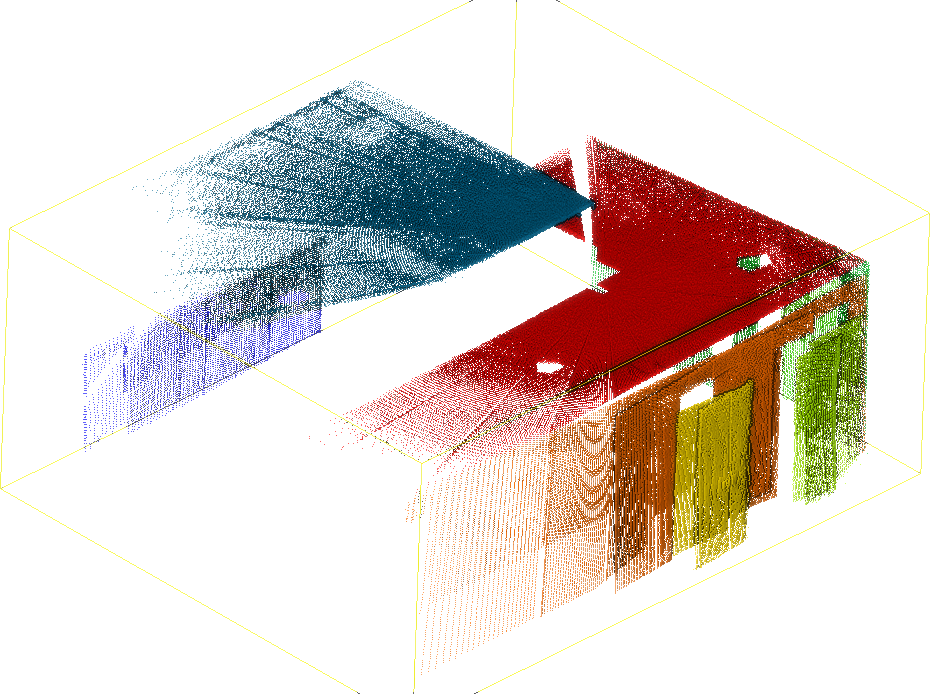
\includegraphics[width=8cm]{images/segmented-pointcloud}
    \caption{Example of a plane segmentation, where each color represents a cluster.}
    \label{figure:cluster-segmentation-1}
\end{figure}

After the segmentation, the calibration procedure can be performed. The plane equation for each point cluster is computed using the Principal Component Analysis method, or PCA. First, the centroid $\bar{p}$ of each plane is found, which is the same as the mean value of all the points $p: (x, y, z) \in \mathds{R}^3$:

\begin{equation}
    \bar{p} = \sum_{i}{p_i}.
        \label{eqn:centroid-plane}
\end{equation}

The covariance matrix $\mathcal{C}$ is then calculated:
%
\begin{equation}
    \mathcal{C} = \sum_{i}{(p_i - \bar{p}) \otimes (p_i - \bar{p})},
        \label{eqn:covariance-matrix}
\end{equation}
%
\noindent where $\otimes$ is the outer tensor product.

Then, the principal axes of the plane are found by an eigendecomposition of the covariance matrix. The smallest eigenvalue $\lambda_3$ will be the variance $\sigma^2$ of the cluster. In other words, $\sigma^2$ is the mean square of the orthogonal distance of all points in the cluster to the plane. So, $\sigma^2$ can be a quantitative factor to measure the cost or each cluster. Formally, let us admit that the $\sigma^2$ has two components: the statistical error of the laser sensor $\sigma^2_{sensor}$, which is not affected by the calibration and a second component $\sigma^2_{calib}$, which depends on the calibration error. Thus, the idea is that, by minimizing $\sigma^2$, an exact calibration can be obtained. For this calibration, however, the value $\sigma$ was used instead of $\sigma^2$, which is known as the Root Mean Square Deviation, or RMS. Therefore, the loss of each cluster will be the $\sigma$ value.

The principal axes of the plane are found by the eigenvalue decomposition of the covariance matrix $\bm{C}$. According to the PCA method, each eigenvalue represents the statistical deviation of the points in each principal axis, more specifically, the mean square error. Therefore the deviation, or statistical error, of each point cluster $\bm{C}_i$ to the corresponding plane $\sigma_i$ is determined by the smallest eigenvalue $\lambda_3$. The cost function can the sum of all $\sigma_i$, according to:
%
\begin{equation}
    \textrm{f} = \sum_{i}^{N}{\sigma_i}.
\end{equation}

\subsection{Optimizer}

The optimization algorithm chosen was Powell's method, described in \cite{powell64}. This method finds a local minimum of a multi-dimensional unconstrained function and does not require the gradient of this function (which is not known is this problem), which fits this particular optimization. This method is implemented in the python scientific library SciPy. However, this method requires multiple evaluations of the objective function at each iteration, in order to calculate an approximate Jacobian matrix in the neighborhood of each point. This usually results in slow optimizations, compared to other methods, such as Gradient Descent.

%%%%%%%%%%%%%%%%%%%%%%%%%%%%%%%%%%%%%%%%%%%%%%%%%%
\section{Results}
\label{section:results}
%%%%%%%%%%%%%%%%%%%%%%%%%%%%%%%%%%%%%%%%%%%%%%%%%%

In this section, the proposed method for the calibration was evaluated using acquired data from a real scene. 

The hardware infrastructure used in this work to acquire the data was the 3D scanner \textit{lemonbot}, show in \cref{figure:lemonbot}. The principal components of this 3D scanner are the PTU \textit{FLIR PTU-D46} and the 2D laser scanner \textit{Hokuyo UTM30LX}\footnote{The 3D scanner, as seen in the \cref{figure:lemonbot}, has two laser scanners: the \textit{Hokuyo UTM30LX} and the \textit{SICK LMS100}. In this work, only the first was used.}. The LRF was mounted on the PTU, to have the scan plane in the vertical direction. The laser scanner can cover \SI{270}{\degree} with an angular resolution of \SI{0.25}{\degree}. The PTU has an angular resolution of \SI{0.0032}{\degree}, so the error in the transformation $^{m}\mathbf{T}_{e}$ (see \cref{equation:point-reconstruction}) is negligible. This 3D scanner was programmed using the \textit{ROS} framework, which handles the hardware drivers, the transformation graph and the recording of the scanning data.

\begin{figure}[h]
    \centering
    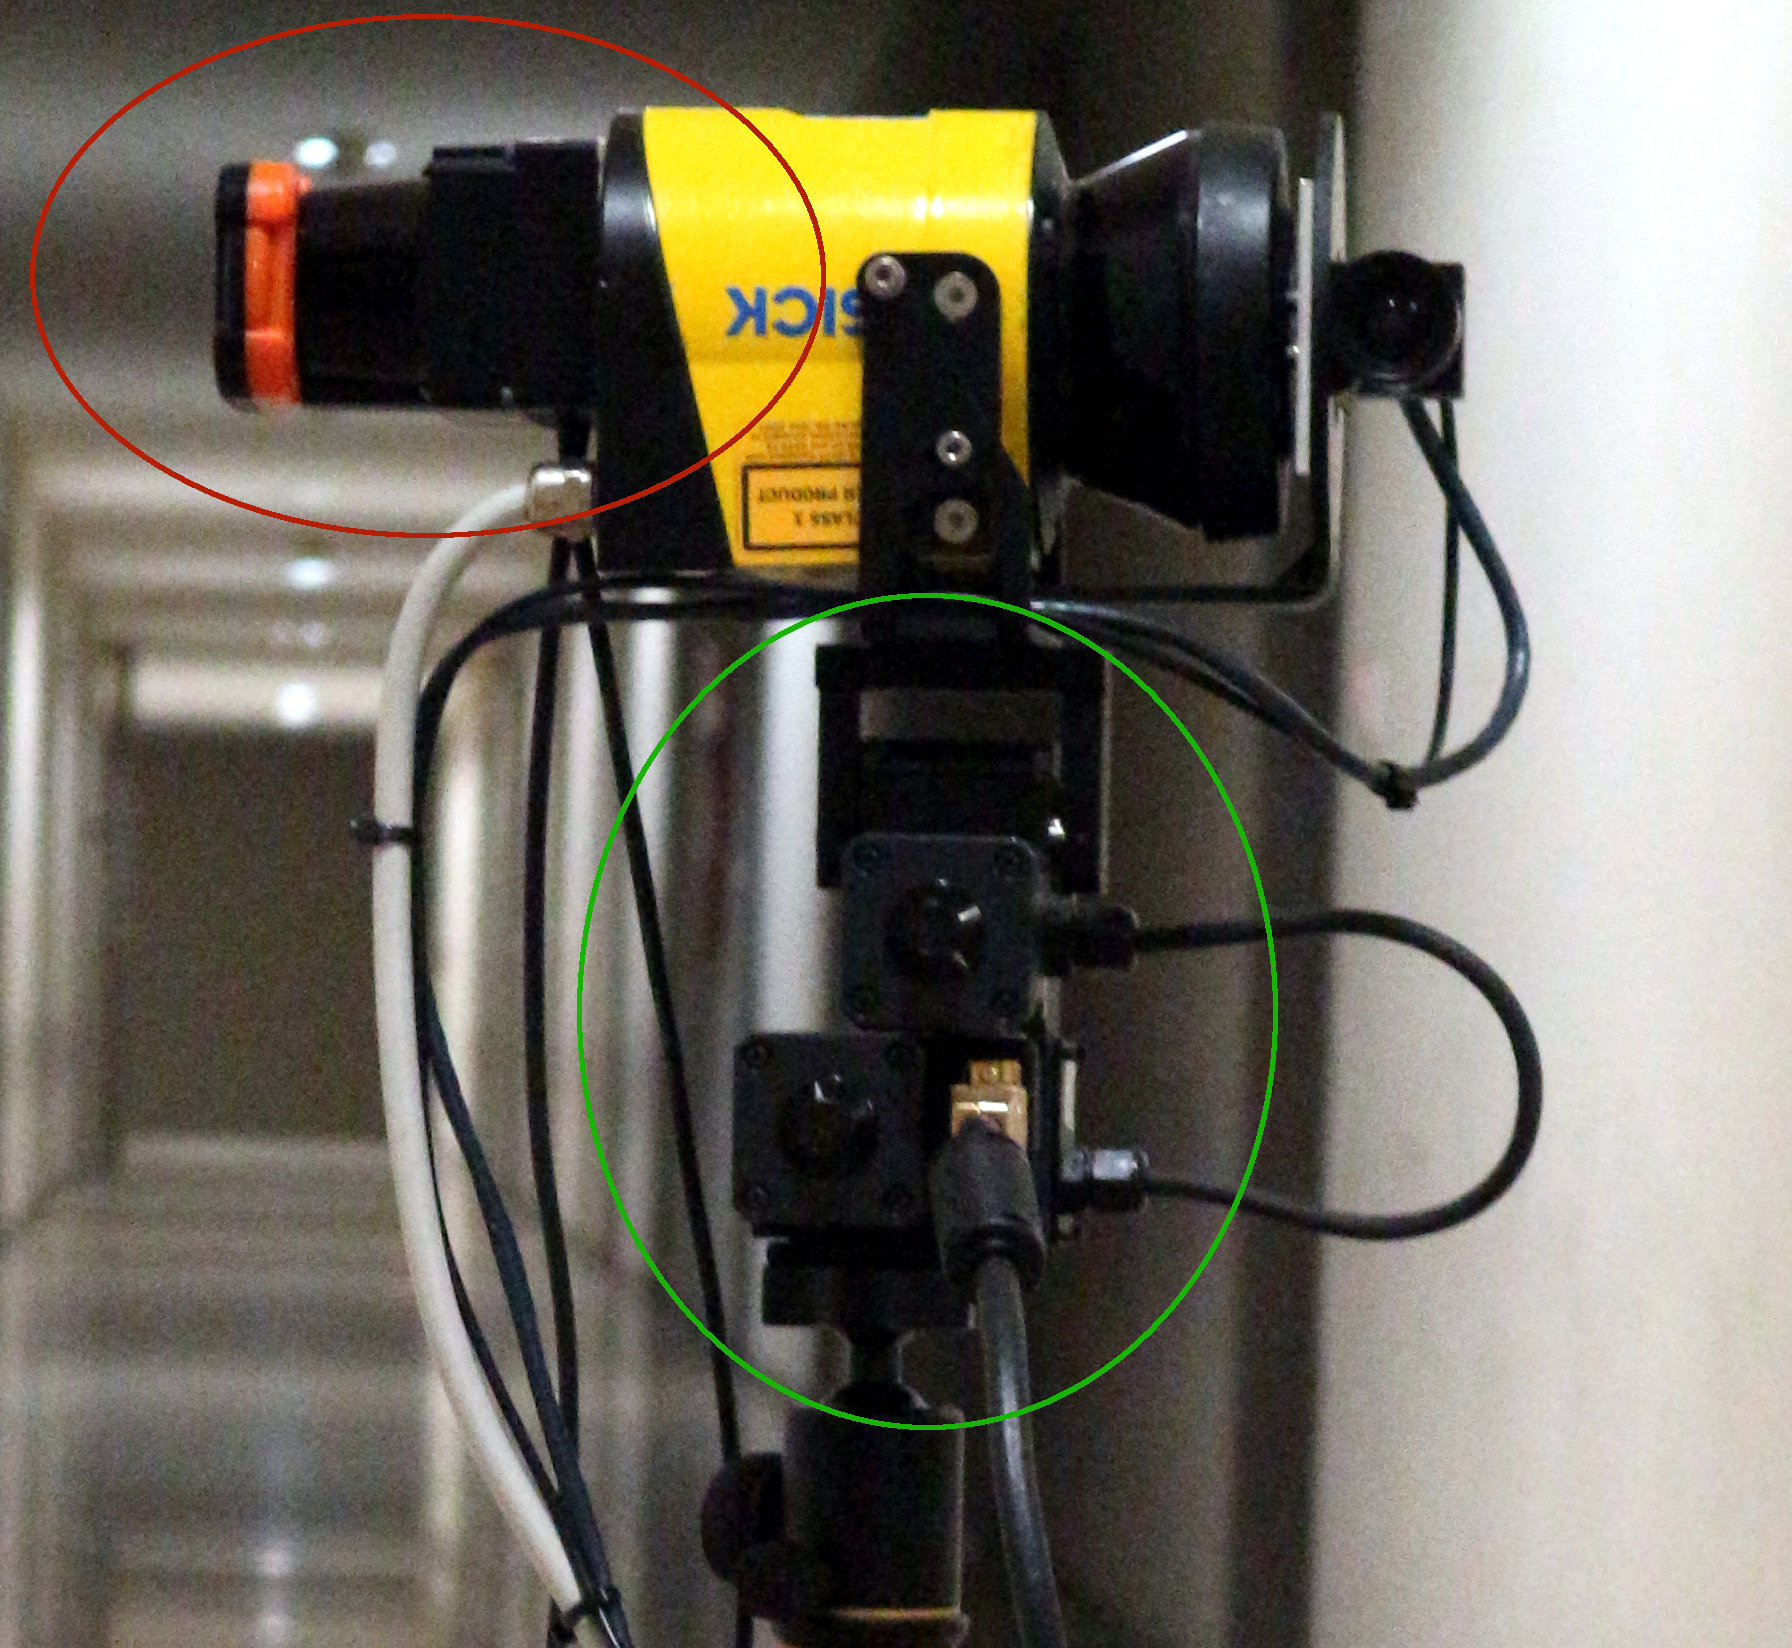
\includegraphics[width=8cm]{images/lemonbot-head}
    \caption{The \textit{lemonbot} 3D scanner, used in this work. The LRF \textit{Hokuyo UTM30} is marked in red and the \textit{FLIR PTU-D46} is marked in green.}
    \label{figure:lemonbot}
\end{figure}

For the verification, a dataset was acquired from a single room, which consists of 3 acquisitions\footnote{One acquisition corresponds to a set of laser scans taken from a particular position in the scene. Each acquisition is processed and results in a point cloud.}. The acquisitions were performed in different positions in the room. The room was not cluttered and the ceiling, walls, and floor are all perpendicular and known to be planar surfaces. This was ensured in order to minimize segmentation and calibration errors.

The optimization procedure was successful minimizing the objective function in every dataset, as seen in \cref{table:iteration-results}. The final results in a qualitative improvement in comparison to the uncalibrated point cloud, as shown in \cref{figure:visual-comparison}. These examples show the most common defects shown in poorly calibrated reconstructions. In the first example, the roof surface appears as multiple unaligned surfaces. This effect can be also seen in a wall, in the third example, which appears in duplication. The second example shows a deformation, which evidently deformed the corner structure in the point cloud. These deformations found in the uncalibrated point clouds are almost imperceptible in the calibrated point cloud.

Practical experience shows that this calibration is resilient to the initial parameters. In this calibration, the initial parameters were roughly determined by visual inspection of the 3D scanner. 

\begin{figure}
    \centering
    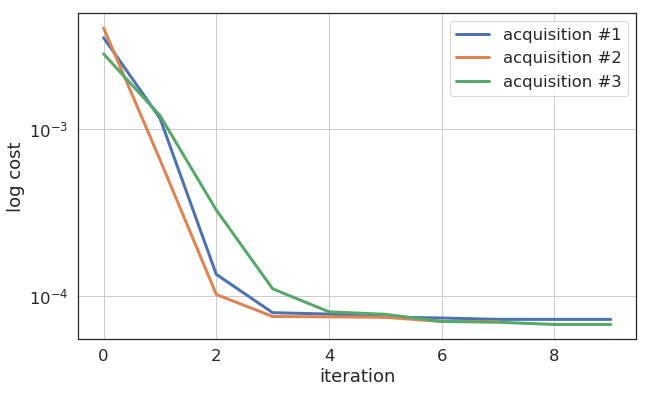
\includegraphics[width=8cm]{images/calibration-evolution.png}
    \caption{Graph of the evolution of the cost function during the optimization process. As seen, the cost function decreased roughly 50 times.}
    \label{table:iteration-results}
\end{figure}

\begin{figure*}
    \centering

    \centering
    \subfloat{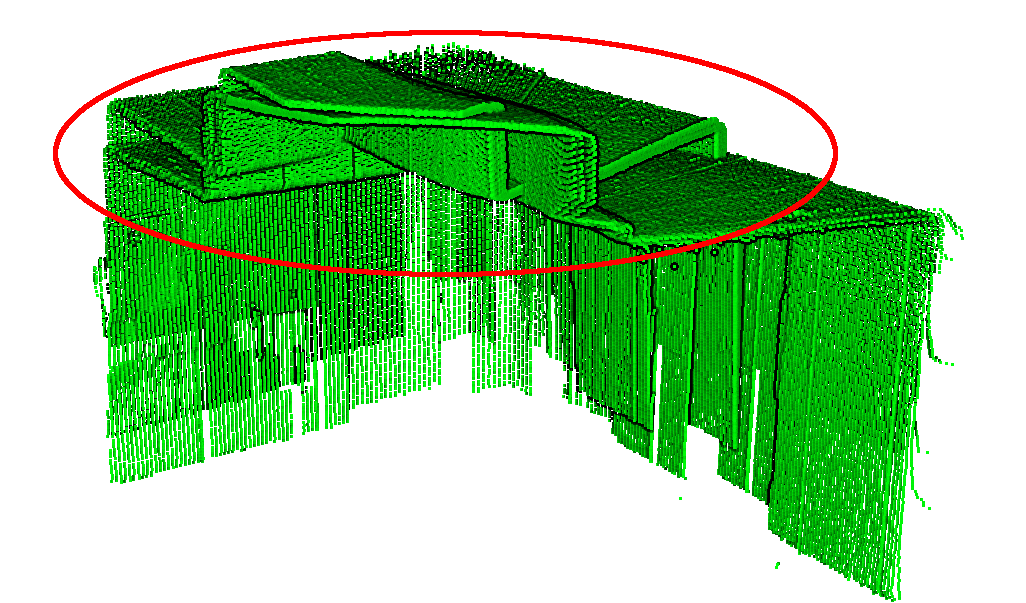
\includegraphics[width = 8cm]{images/example-pointcloud-2-bad}} \qquad
    \subfloat{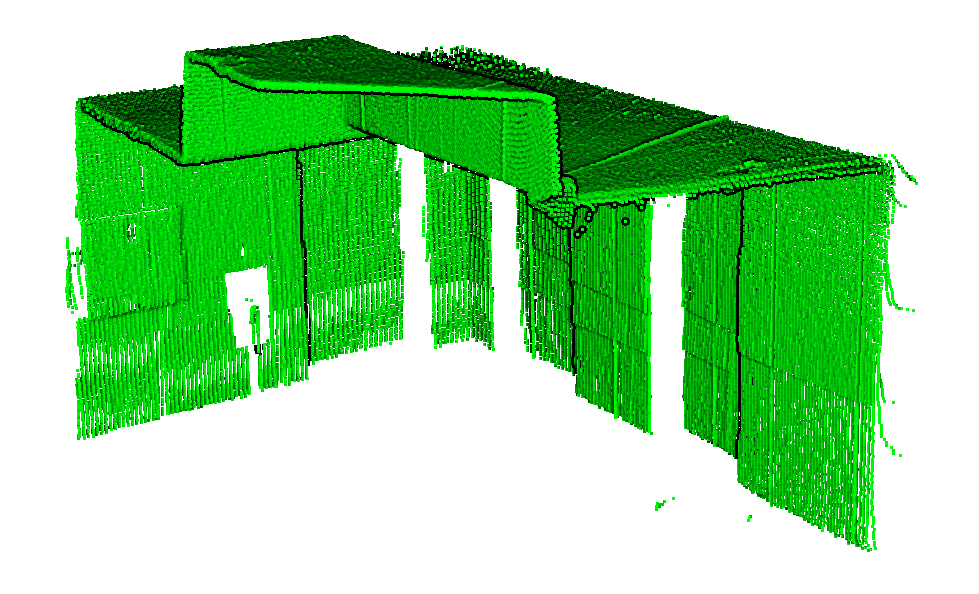
\includegraphics[width = 8cm]{images/example-pointcloud-2-good}}

    \centering
    \subfloat{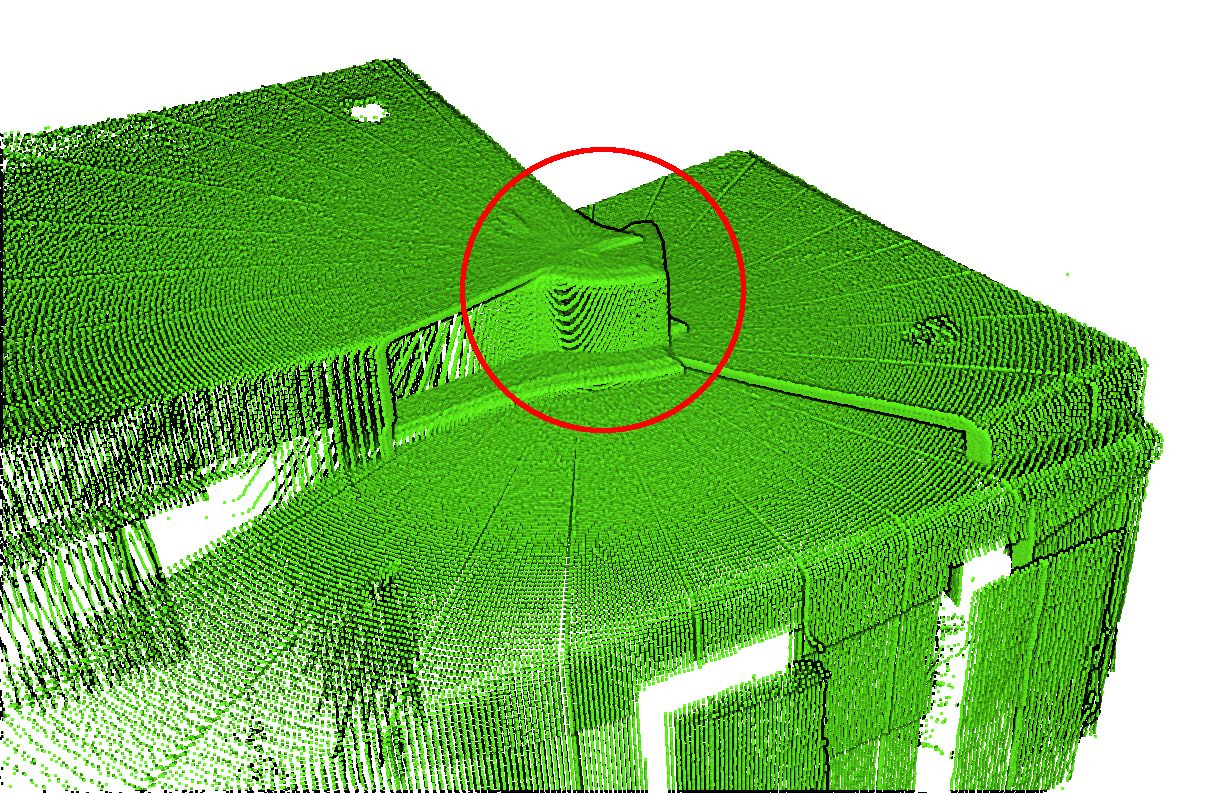
\includegraphics[width = 8cm]{images/example-pointcloud-3-bad}} \qquad
    \subfloat{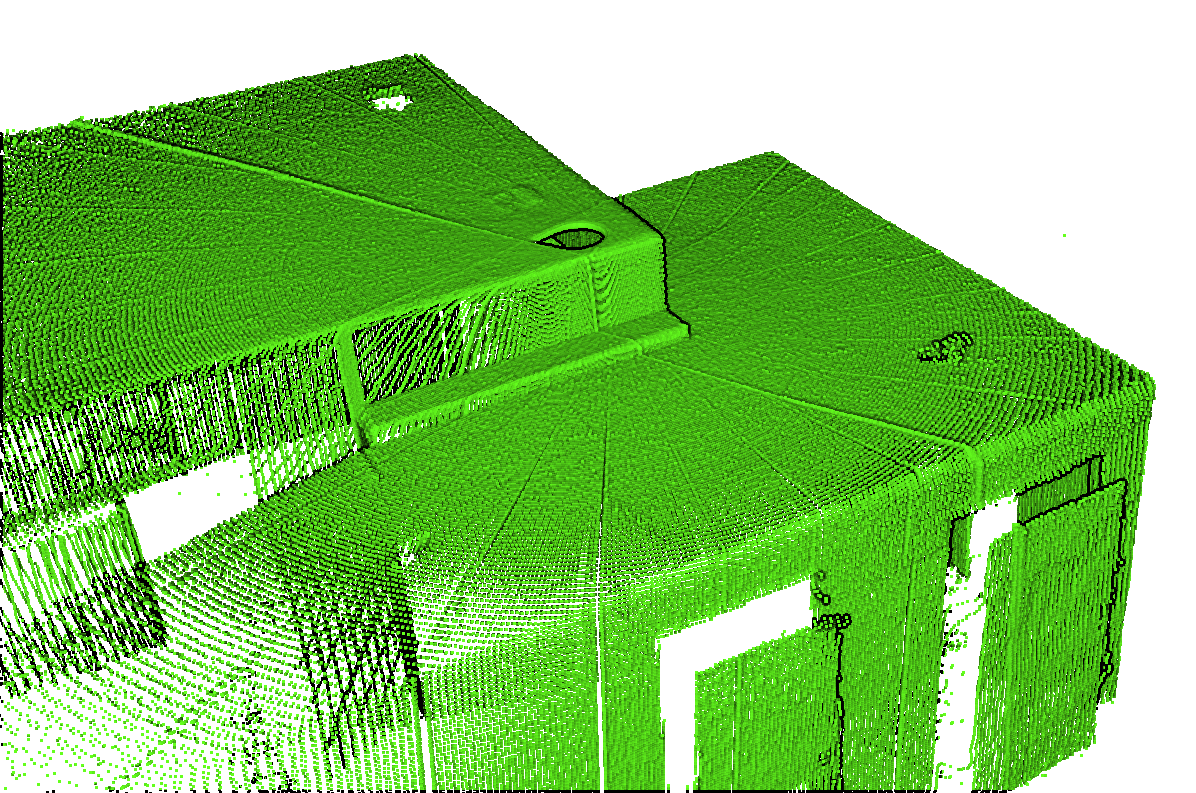
\includegraphics[width = 8cm]{images/example-pointcloud-3-good}}

    \centering
    \subfloat{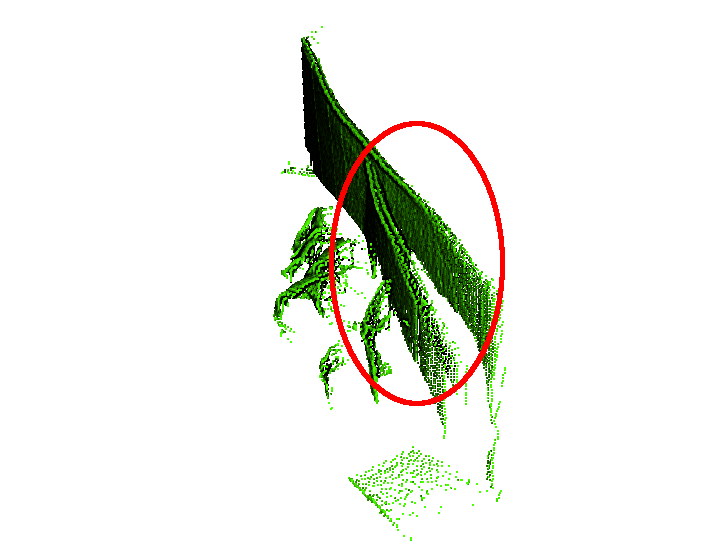
\includegraphics[height = 6cm]{images/example-pointcloud-1-bad}} \qquad
    \subfloat{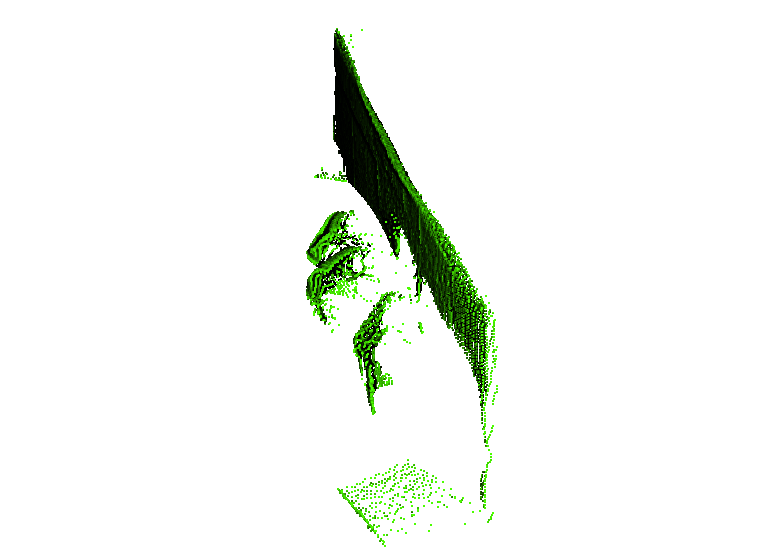
\includegraphics[height = 6cm]{images/example-pointcloud-1-good}}

    \caption{Side-by-side comparison of the uncalibrated (left) and calibrated (right) point clouds. The most noticeable distortions are marked in the uncalibrated point clouds and do not appear in the respective calibrated point clouds. This indicates that the method successfully reduces the distortions in the point clouds.}
    \label{figure:visual-comparison}
\end{figure*}

Despite the good qualitative result, a further quantitative analysis was performed in order to evaluate the method. The results were prepared in the following steps:

\begin{itemize}
    \item A planar surface was extracted from both the calibrated and uncalibrated point cloud.
    \item The fitting plane was calculated for each surface, and the distance between the points to the surface was computed.
    \item The statistic deviation of the distances was calculated.
\end{itemize}

This method was performed for 3 manually segmented planes, such as the ones seen in \cref{figure:cluster-segmentation-1}, and the segments can be seen in \cref{table:quantitative-results}. As seen the statistical deviation is, in fact, smaller in the calibrated point cloud. As an alternative view, in \cref{figure:deviation-histogram}, the histogram, and distribution of the signed deviation are shown for both the point clouds. As shown, the deviations of the calibrated point cloud are less scattered than the deviations of the uncalibrated point cloud. These results indicate that this calibration method, in fact, improves the results. 

\begin{table}
    \caption{Comparison between the standard deviation and mean of the distances of the points to the plane for both the calibrated and uncalibrated point clouds.}
    \begin{tabu}{X[l] X[c] X[c]}
        \toprule
                       & $\mu / \si{\meter}$ (average) & $\sigma / \si{\meter}$ (std. dev.) \\
        \midrule
        Calibrated     & 0.0495 & 0.2589 \\
        Uncalibrated   & 0.0025 & 1.1211 \\
        \bottomrule
    \end{tabu}

    \label{table:quantitative-results}
\end{table}

\begin{figure}[h]
    \centering
    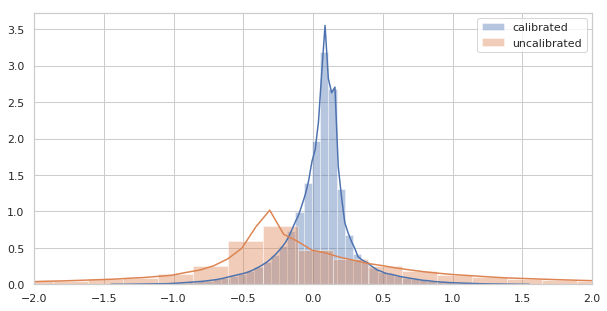
\includegraphics[width=8cm]{images/pointclouds-histogram.png}
    \caption{Distribution of the distances of the points to the plane. The uncalibrated points is wider than the calibrated points, which indicates that the calibration improved the reconstructed point cloud.}
    \label{figure:deviation-histogram}
\end{figure}


%%%%%%%%%%%%%%%%%%%%%%%%%%%%%%%%%%%%%%%%%%%%%%%%%%
\section{Conclusions and Future Work}\label{sec:conclusions}
%%%%%%%%%%%%%%%%%%%%%%%%%%%%%%%%%%%%%%%%%%%%%%%%%%

This paper presents a calibration procedure to determine the extrinsic transformation of 2D-LRF and PTU. The accuracy of this transformation is critical for multiple applications, of which the most noticeable are 3D reconstruction systems. The incorrect calibration of these systems results in artifacts and deformations on the final reconstructions, which invalidates any successive work in these point clouds. The proposed method is based on the measurement of the deformations of reconstructed planar surfaces, and through an optimization procedure, these deformations are minimized. The method was proved to be effective, through a visual inspection of the resulting point cloud and through statistical evaluation of the reconstructed geometries.

Further work can be done in order to improve or validate further this algorithm, such as: a study of a automatic segmentation procedure; the determination of the Jacobian of the cost function, in order to reduce the iteration time of the optimization, by enabling new optimization methods, such as the gradient descent; the validation of this method with data using different 2D-LRF and different dynamic kinematic chains, such as a robotic arm; the comparison of the point cloud generated with this reconstruction method with point clouds generated with high-end commercial 3D scanners, such as the \textit{FARO Focus 3D}; and study the impact of the calibration environment (for example, the number and pose of the planes and size of the room) in the calibration accuracy.


\bibliographystyle{IEEEtran}
\bibliography{references/refs}


\end{document}
